
\documentclass[12pt]{article}
\usepackage[a4paper, margin=.30in]{geometry}
\usepackage{graphicx ,
            wrapfig,
            xcolor, 
            enumerate,
            amsmath,
			fontenc,
			tcolorbox
            }

\newcommand\headerMe[2]{\noindent{}#1\hfill#2}
\renewcommand{\thesection}{\Roman{section}}

\author{Zakaria HAOUZAN}
\date{\today}

\begin{document}
% headers --------------
\headerMe{Matière : Physique-Chimie}{Professeur : Zakaria HAOUZAN}\\
\headerMe{Unité : Ondes }{Établissement : Lycée SKHOR qualifiant}\\
\headerMe{Niveau : 2BAC-SM-X}{Heure : 5H}\\

% ------Content ________
\begin{center}

    \Large{Leçon $N^{\circ} 1 $: \color{red}Ondes mécaniques progressives. }
\end{center}

%\begin{wrapfigure}[10]{r}{0.5\textwidth}
%    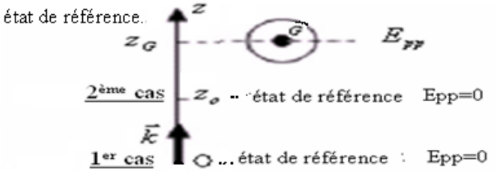
\includegraphics[width=0.5\textwidth]{./img/img00.png}
%\end{wrapfigure}


\section{ Définition d’une onde mécanique : }

On appelle onde mécanique le phénomène de propagation d’une perturbation dans un milieu matériel élastique, sans transport de la matière,mais avec transport d'énergie.
\section{ Ondes longitudinales, transversales, et leurs caractéristiques. }

L'onde est transversale si la déformation du milieu matériel est perpendiculaire à la direction de sa propagation.

L'onde est longitudinale si la déformation du milieu matériel est parallèle à la direction de sa propagation.


\subsection{Propagation d'une onde mécanique le long d'une corde:}
On provoque une perturbation verticale à l'une de ses extrémités d'une corde élastique tendue horizontalement. On constate que la perturbation se propage le long de la corde comme l'indique la figure suivante:
\begin{wrapfigure}[4]{r}{0.5\textwidth}

	
	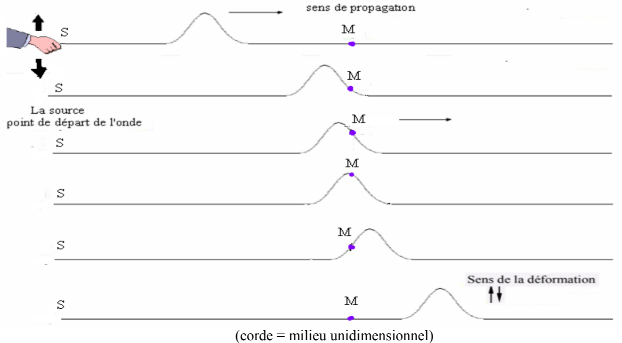
\includegraphics[width=0.5\textwidth]{./img/Corde Propagation.png}
	\caption{Propagation d'une onde mécanique le long d'une corde (corde:milieu unidimensionnel)}
\end{wrapfigure}


\begin{itemize}
	\item La propagation d'une onde mécanique nécessite un milieu matériel (gaz, liquide ou solide).
	\item Dans la cas précédent, la corde qui est milieu de propagation est un milieu matériel, donc il s'agit d'une onde mécanique.
	\item Chaque point M de la corde , lorsque l'onde l'atteint se déplace verticalement (perpendiculairement) à la direction de
propagation : l'onde est donc transversale.
\item Après le passage de l'onde, chaque point M de la corde reste à sa place, donc lors de sa propagation l'onde ne transporte pas la
matière mais elle transporte l'énergie.

\end{itemize}

\begin{wrapfigure}[4]{r}{0.2\textwidth}	
	\vspace{-2cm}
	
\includegraphics[width=0.2\textwidth]{./img/POM_surface de l'eau.png}
	\caption{Propagation d'une onde mécanique dans l'eau}
\end{wrapfigure}
\subsection{Propagation d'une onde mécanique à la surface de l'eau:}
On provoque une onde circulaire à la surface de l'eau en jetant une pierre dans l'eau (milieu bidimensionnel).

On constate que le morceau de liège placé à la surface de l'eau lorsque l'onde l'atteint se déplace verticalement et il reste à sa
place après le passage de l'onde: donc il s'agit d'une onde mécanique transversale.

\subsection{Propagation d'une onde mécanique le long d'un ressort :}

On comprime quelques spires à l'une des extrémités d'un ressort tendu horizontalement sur une table puis on les lâche brusquement.

\begin{wrapfigure}[4]{r}{0.3\textwidth}	
	%\vspace{2cm}
	\caption{Propagation d'une onde mécanique dans l'eau}
	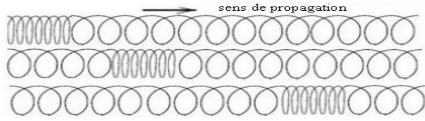
\includegraphics[width=0.3\textwidth]{./img/POM_ressort.png}
\end{wrapfigure}
On constate la propagation de l'onde le long du ressort parallèlement à la direction de propagation, donc il s'agit d'une onde
mécanique longitudinale. (Le ressort=milieu matériel unidimensionnel)


\subsection{Les Ondes sonores :}
\begin{figure}[h]
		\begin{center}
	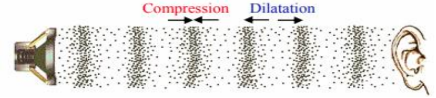
\includegraphics[width=0.4\textwidth]{./img/OndeSonore.png}
	\vspace{-0.5cm}
	\caption{Onde mécanique longitudinale (onde sonore)}
\end{center}
\end{figure}
\begin{itemize}
	\vspace{-1.3cm}
\item Le son est une onde mécanique longitudinale tridimensionnelle: sa propagation nécessite la présence d'un milieu materiel ( l'air par exemple mais aussi n'importe quel milieu gazeux, liquide ou solide.)
\item Le son ne se propage pas dans le vide (absence de la matière)..
\item La propagation du son est due à la compression et la dilatation des constituants du milieu de propagation.
\end{itemize}

\subsection{Vitesse de propagation d'une onde :}
\subsubsection{Définition : }
\begin{tcolorbox}
	
	\textit{La vitesse de propagation d'une onde (nommée célérité) est égale à la distance parcourue au temps mis à la parcourir.$$v = \frac{d}{\Delta{t}}$$
	Remarque:	La vitesse du son dépend du milieu de propagation.Elle est plus importante dans les solides et les liquides que dans l'air.}

\end{tcolorbox}
\subsubsection{Cas de propagation le long d'une corde : }
La vitesse de propagation d'une onde le long d'une corde tendue est donnée par la relation suivante: $$ v = \sqrt{\frac{T}{\mu}}$$

T: tension de la corde en (N).
et $\mu$ : masse Linéaire de la corde en (Kg/m), avec $\mu = \frac{m}{L}$

\subsubsection{Exemple d'application:}
Une onde se propage le long d'une corde tendue de masse m=100g et de longueur l=8m et sa tension T=5N.
\\1. Calculer la vitesse (célérité) de propagation de l'onde.
\\2. Quelle est le temps mis par l'onde pour parcourir la corde toute entière ?
\begin{wrapfigure}[4]{r}{0.3\textwidth}	
			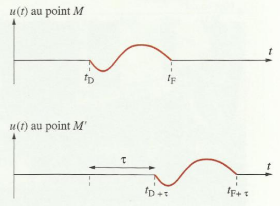
\includegraphics[width=0.3\textwidth]{./img/RetardCourbe.png}
			\caption{Onde mécanique longitudinale}
\end{wrapfigure}
\section{Notion de retard temporaire :}
\begin{itemize}	
	\item Désignons par $u$ les valeurs du déplacement transversale provoqué par une onde se propageant le long d'une corde.

	\item les graphiques du document 17 représentent la perturbation $u$ en fonction du temps en un point M de la corde, puis en un point M'.

	\item la perturbation $u$ se propage à la vitesse $v$, elle affecte le point M' à partir de la date $t_D$ (D comme début de la perturbation), puis le point M' à partir la date $t_D+\tau$.
\item $\tau$ désigne le retard du passage de la déformation en M', par rapport à M. On a $v = \frac{MM'}{\tau}$.
\end{itemize}
Remarque:

\begin{tcolorbox}
\begin{wrapfigure}[8]{r}{0.3\textwidth}	
			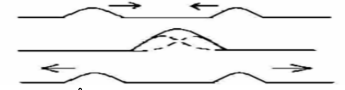
\includegraphics[width=0.3\textwidth]{./img/eux ondes mécaniques se croisent.png}
			\caption{deux ondes mécaniques }
\end{wrapfigure}
	La relation entre l'élongation d'un point M du milieu de propagation et celle de la source est : $$u_M(t) = u_S(t-\tau)$$ avec $\tau = \frac{SM}{v}$

	Lorsque deux ondes mécaniques se croisent elles se superposent sans se perturber. (Leurs amplitudes s'ajoutent algébriquement)
et après leur croisement chaque onde reprend sa forme propre et continue sa propagation avec sa même vitesse.

\end{tcolorbox}

\section{Exercice d’application 2:}
Une onde mécanique est engendrée à la date $t=0s$, à l’extrémité d’une corde, elle se propage à une célérité $v = 5m.s^{-1}$

Nous considérons les points M , N et P de la corde telles que: $SM=10m$, $SN=12m$, $SP=15m$.

Sachant que la durée de perturbation est $\Delta{0.2s}$, décrire l’état de ces points à l’instant $t=2.5s$



%wfg---------------------------------------------------------------sf 
%\begin{center}
   %\begin{tabular}{ |c|c|c|c|c|c|c| }
      %\hline
      %km & hm & dam & \bf{m} & dm & cm & mm \\
      %\hline
        %&   &    &  &   &   & \\
%\hline
%\end{tabular}
%On place un seul nombre dans chaque case.
%\end{center}
%\begin{center}
   %\begin{tabular}{ |c|c|c|c|c|c|c| }
      %\hline
      %$km^2$ & $hm^2$ & $dam^2$ & \bf{$m^2$} & $dm^2$ & $cm^2$ & $mm^2$ \\
      %\hline
        %&   &    &  &   &   & \\
%\hline
%\end{tabular}
%\end{center}


\end{document}

